%
% File acl2014.tex
%
% Contact: koller@ling.uni-potsdam.de, yusuke@nii.ac.jp
%%
%% Based on the style files for ACL-2013, which were, in turn,
%% Based on the style files for ACL-2012, which were, in turn,
%% based on the style files for ACL-2011, which were, in turn, 
%% based on the style files for ACL-2010, which were, in turn, 
%% based on the style files for ACL-IJCNLP-2009, which were, in turn,
%% based on the style files for EACL-2009 and IJCNLP-2008...

%% Based on the style files for EACL 2006 by 
%%e.agirre@ehu.es or Sergi.Balari@uab.es
%% and that of ACL 08 by Joakim Nivre and Noah Smith

\documentclass[11pt]{article}
\usepackage{acl2014}
\usepackage{times}
\usepackage{url}
\usepackage{latexsym}
\usepackage{amsmath}
\usepackage{amsfonts}
\usepackage{amssymb}
\usepackage{color}
%\DeclareMathOperator*{\argmax}{arg\,max}
%\DeclareMathOperator*{\argmin}{arg\,min}

\usepackage{graphicx}
\usepackage{xspace}
\usepackage{multirow}


%\setlength\titlebox{5cm}

% You can expand the titlebox if you need extra space
% to show all the authors. Please do not make the titlebox
% smaller than 5cm (the original size); we will check this
% in the camera-ready version and ask you to change it back.
%\input{defs}

\title{Parameter Agreement Training with and without Parallel Data}
%{Joint Training of Alignment Models: with and without Parallel Data}


%\author{First Author \\
%  Affiliation / Address line 1 \\
%  Affiliation / Address line 2 \\
%  Affiliation / Address line 3 \\
%  {\tt email@domain} \\\And
%  Second Author \\
%  Affiliation / Address line 1 \\
%  Affiliation / Address line 2 \\
%  Affiliation / Address line 3 \\
%  {\tt email@domain} \\}
%\date{}

\input{math_definition.tex}

\begin{document}
\maketitle
\begin{abstract}
Learning how to align sequences is a key problem in NLP.
Most approaches model alignment as a directed generative process by which an observed target sequence arises from an observed source sequence. 
In word alignment in particular, symmetrizing inferences of models trained in both directions (source-to-target and reverse) leads to improved alignments.
\marginpar{DC: Something needs to be said here about bidirectionality, or it doesn't make sense. \bluetext{TL: fixed}}
We propose an unsupervised approach for jointly learning bi-directional alignment models by means of maximizing their data likelihoods as well as a measure of model agreement.
In contrast to the ``alignment by agreement'' approach of Liang et al., our method is applicable even without parallel data.
We test our method on two different tasks.
On Czech-English and Chinese-English word alignment, 
we gain 0.4-0.5 BLEU compared to GIZA++ which, Combined with alignments from Liang et al.'s model brings the total improvement to +0.8 $\pm$ 0.1 BLEU.
On a Japanese-to-English back-transliteration task \emph{without} parallel data, our method, when applied to the decipherment model of Ravi and Knight, learns sparser models that reduce whole-name error rate by 33\% relative to a model trained on parallel data.
\end{abstract}

\section{Introduction}
\label{sec:introduction}
\iffalse
Many tasks in machine translation (MT) are first approached by modeling the transfer of information from one language to another (say, English to French). 
The resulting directional models often follow a simple generative story that explains how source language entities could have generate corresponding target language entities. 
For example, the IBM word alignment models \cite{Brown1993} explain how strings composing an English sentence can be translated and rearranged (distorted) into strings composing a French sentence and pronunciation Finite State Transducer (FST) can be used to explain how names in English undergo phonetic changes as they are uttered in French.

However, the directionality may come with a price, as it impose restriction on the inference space - in the word alignment models (IBM 1 or 2 and HMM), only one-to-many word alignments (target to source) are possible, which may not fit well for some language pairs (for example, German compound target words usually arise from multiple English source words). 
For this reason, it is common practice to produce word alignment inferences using models trained in both directions and then apply a post-processing symmetrization technique (such as grow-diag-final-and).
However, while post-processing resolves some of the problems, independent training can still lead the two models to divergent local maxima; ones whose disagreeing inferences cannot be fixed by post-processing techniques.

In Alignment by Agreement (ABA), Liang et al. (2006) suggest to jointly train the two directional models, each maximizing its own data likelihood (as would be done independently) as well as a model coupling term that encodes some measure of agreement between the models.
Their suggested agreement measure further exploits the observed parallel training data by rewarding similarity between the two alignment posteriors (one for each direction) computed on each training sentence pair.
Indeed, their experimental results show that training with posterior agreement leads to better performing models (reduced AER). At the same time however, the ABA formulation cements the dependency on parallel data thus limiting the applicability of their method to other settings.

In this paper, we present Parameter Agreement Training (PAT); a method that operates with a different measure of agreement in mind (Section \ref{sec:model}))
Remaining in context of word alignment (as we have so far), the general idea is as follows: Consider the two directional word alignment models' translation tables. 
For any bilingual pair of words $e$ and $f$, it seems reasonable that $t(f \mid e)$ is high/low whenever $t(e \mid f)$ is high/low.
This intuition follows simply since word translation is generally invertible \footnote{The word $e$ should be in the set of translations of the translation of $e$}.
With the above in mind, we designed an agreement measure that encourages agreement in the two directional models parameters magnitudes.
Our resulting objective function can be optimized using EM, where the E-step remains unchanged and the M-step reduces to an instance of convex programming.

Furthermore, our new agreement measure is free of the parallel data dependency which in turn broadens the range of settings our method can be applied to beyond conventional word alignment.
In particular, our method can be applied in the challenging decipherment setting, under which no parallel data is provided.

We conduct two sets of experiments (Section \ref{bla}): (1) Our word alignment experiments (with parallel data) show comparable F- and BLEU score improvements to those of ABA on various language pairs.
Combining the phrase-tables of both ABA and PAT leads to further increase in BLEU score.
(2) In the decipherment settings (without parallel data) we repeat the Japanese to English back-transliteration experiments as described by Ravi and Knight (2009?). 
PAT nearly splits the difference between the baseline (Ravi and Knight's formulation) and a method trained using parallel data. 
Finally, ... ?
\fi

Alignment is a crucial subtask for many larger NLP problems: Word alignments are the backbone for extracting translation rules used in statistical machine translation; phoneme alignments are used to transliterate words in one language to another. The goal is to align entities, which could be words or phonemes, between two sequences, which could be pairs of source and target sentences, for example French and English sentences, or pairs of phoneme sequences, for example English phoneme and Japanese katakana sequences. 

The popular models used in these tasks are both \emph{generative} and \emph{directed}, that is, they define a directed sequence of events by which one side of the pair produces the other side. For example, the IBM models for word alignment \newcite{brown+alii:1993} describe a stochastic process by which the target sentence is generated from the source sentence via word alignments. These processes can sometimes produce different alignments, depending on the direction of generation. However, the directionality may come with a price, as it impose restriction on the inference space - in the word alignment models (IBM 1 or 2 and HMM), only one-to-many word alignments (target to source) are possible, which may not fit well for some language pairs (for example, German compound target words usually arise from multiple English source words). To remedy this, we resort to ad-hoc alignment symmetrization approaches , such as grow-diag-final-and \cite{koehn+:2003}, \emph{after} training. However, while post-processing resolves some of the problems, independent training can still lead the two models to divergent local maxima; ones whose disagreeing inferences cannot be fixed by post-processing techniques. 

A second problem for training alignment models is the need for parallel data. For example, in \newcite{KG98}, the authors use (some number) \marginpar{insert number} of parallel English-Katana sequences to training phoneme alignment models. While large amounts of parallel data needed for word alignment is readily available for many language pairs, acquiring parallel phoneme sequences for transliteration can be very challenging. 

There has been previous work on solving the problem of model disagreement \cite{liang+:2006:align} (ABA), and training phoneme alignment models with monolingual data \cite{RK09}. \newcite{liang+:2006:align} suggest an approach, Alignment by Agreement (ABA), to jointly train the two directional models, each maximizing its own data likelihood (as would be done independently) as well as a model coupling term that encodes some measure of agreement between the models. Their suggested agreement measure further exploits the observed parallel training data by rewarding similarity between the two alignment posteriors (one for each direction) computed on each training sentence pair. Indeed, their experimental results show that training with posterior agreement leads to better performing models (reduced AER). However, in \newcite{liang+:2006:align}, the authors do not optimize a clear objective function and their approach cannot be applied to training alignment models without parallel data. For phoneme alignment, \newcite{RK09} alleviate the reliance on parallel data and improve monolingual alignment quality over the baseline, but their approach does not encourage model agreement, which can further improve alignment accuracy, as we will show in section~\ref{sec:results}. 

In our paper, we present a \emph{single} approach that achieves both model agreement during training, and can be used in non-parallel settings. Our approach, Parameter Agreement Training (PAT), operates with a different measure of agreement in mind (Section \ref{sec:model})). The general idea can be easily illustrated in the word alignment setting: Consider the two directional word alignment models' translation tables.  For any pair of words $e$ and $f$, it seems reasonable that $t(f \mid e)$ is high(low) whenever $t(e \mid f)$ is high(low). This intuition follows simply since word translation is generally invertible \footnote{The word $e$ should be in the set of translations of the translation of $e$}.
With the above in mind, we design an agreement measure that encourages agreement in the magnitudes of the parameters of the models in each direction.
Our resulting objective function can be optimized using EM, where the E-step remains unchanged and the M-step reduces to an instance of convex programming. Furthermore, since our approach encourages agreement between the model parameters, it can be applied in non-parallel settings such as unsupervised phoneme alignment with monolingual data. Using our approach, we are able to significantly improve over \newcite{RK09}, achieving a $50\%$ reduction in error. For word alignment, our results compare favorably with results from previous approaches for model agreement. 

%The generative process for word alignment allows a target word to align to \emph{at most} one source word, producing different alignments in the source-target vs target-source directions.


 
%%%% old introduction
%Word alignment is an important part of any statistical translation pipeline. The most widely used word alignment models are the the IBM \cite{brown+alii:1993} and HMM \cite{vogel+alii:1996} models. These models describe a generative process by which the source sentence ($E$) generates the target sentence ($F$) via one-to-many alignments. The models are trained independently in each direction, and at test time, the alignments from both directions are \emph{symmetrized} using heuristics like \emph{grow-diag-final} \cite{och+ney:2003}. Although symmetrization corrects some of the mistakes that the independently trained models make, \newcite{liang+:2006:align} and \newcite{ganchev2010posterior} show that word alignment quality be improved when the models are trained jointly to agree on their inferences. However, the method of \newcite{liang+:2006:align} relies on parallel data, which might not always be the available, for example, in unsupervised transliteration with non-parallel data \cite{RK09}. Another method, posterior regularization \cite{ganchev2010posterior}, can be expensive, making it difficult to scale to large data. In this paper, we present an approach that improves unsupervised transliteration quality (section~\ref{sec:transliteration}) over a state-of-the-art baseline by jointly training English-Japanese and Japanese-English transliteration models on non-parallel data. Unlike the methods of \newcite{liang+:2006:align} and \newcite{ganchev2010posterior}, our approach encourages agreement in the parameters of the models (sections \ref{sec:background} and \ref{sec:method}). We also apply our procedure on joint training of word alignment models (section ~\ref{sec:alignment}) and we achieve results comparable to those of \newcite{liang+:2006:align} on multiple language pairs. 
%
%\iffalse
%predictions by symmetrization increases the overall predictive performance.
%Several papers address this issue directly by jointly training these
%asymmetric models with a particular notion of agreement in mind {[}reference{]}.
%Generally speaking, these techniques encourage the two models to agree
%on their inferences (posteriors) either on each sentence pair individually,
%or over all sentence pairs together.
%
%{[}{[}However, agreement on inference essentially treats the two models
%themselves as black-boxes{]}{]}
%
%In this paper, we explore a different type of model agreement we call
%parameter agreement... (needs more content)
%
%\fi

\section{Background}
\label{sec:background}
\subsection{Generative Models}
We are concerned with learning generative models that describe transformations of a source-language sequence $\ve$ to a target-language sequence $\vf$.
We consider two different settings for these models.

In the parallel data setting, both $\vx = (\ve, \vf)$ are observed. 
The generative story assigns the following probability to the event that $\vf$ arises from $\ve$:
\begin{equation}
p(\vx; \Theta) = p(\vf \mid \ve) = \sum_\va p(\va,\,\vf \mid \ve)
\label{eqn:parallel}
\end{equation}
where $\Theta$ denotes the model parameters and $\va$ denotes a hidden variable that corresponds to unknown choices taken of the generative process.
%(in our case, $\va$ is an alignment, see next subsection).

In the decipherment setting, only the target entity $\vf$ is observed and the source entity $\ve$ is considered hidden. 
Letting $\vx = (\vf)$ the decipherment model takes the form:
\begin{equation}
p(\vx; \Theta) = p(\vf) = \sum_{\ve} p(\ve) \sum_{\va} p(\va,\,\vf \mid \ve)
\label{eqn:decipherment}
\end{equation}
That is, according to the decipherment generative story, the observed entity $\vf$ can arise from any source entity $\ve$ by first selecting $\ve \sim p(\ve)$ and then proceeding according to the parallel data generative story.

Training these models entails the same objective - maximizing the observed data log-likelihood $L(\Theta \mid X)$:
\begin{align*}
\max_{\Theta}\,\,L(\Theta \mid X)
%=&\max_{\Theta}\,\,\log\prod_{n}p (\vx_n;\Theta)\\
=&\max_{\Theta}\,\,\sum_{n}\log p (\vx_n;\Theta)
\end{align*}
%_{n=1}^{N}
where $X=\set{(\ve_{n},\, \vf_{n})}_n$ in the parallel data setting and $X=\set{(\vf_{n})}_n$ in the decipherment setting.

Next, we make these generative stories concrete by explicitly defining $p(\va, \vf \mid \ve)$ and $p(\ve)$ (if necessary) in two sequence alignment tasks - word alignment and back-transliteration decipherment.

%We make the discussion concrete by discussing two related tasks - word alignment and back-transliteration. 

%The predominant approach for training these generative models 

\subsection{Parallel Data: Word Alignment}

%Keeping the discussion abstract, we consider the general problem of sequence alignment. 
%In sequence alignment, we are given a sequence $e = (e_1, \ldots, e_I)$ comprising of source language entities and a sequence $f = (f_1, \ldots, f_J)$ comprising of target language entities (concretely, these entities can represent words or phonemes in each language) and are tasked with finding an alignment 

Word alignment is one of the major building blocks in the conventional machine translation pipeline.
In word alignment, the entity $\ve = (\ve_1, \ldots, \ve_I)$ represents a sentence in the source language and $\vf = (\vf_1, \ldots, \vf_J)$ represents a sentence in the target language. 
The generative story for the transformation of $\ve$ to $\vf$ follows according to \eqn{eqn:parallel} where the hidden variable $\va = (\va_1, \ldots, \va_J)$ corresponds to a sequence of $J$ indices and encodes an asymmetric \emph{target-to-source} alignment under which the $j$th target word is aligned to the $\va_j$th source word. 
In other words, under the generative story, $\vf_j$ is thought to be generated from $\ve_{\va_j}$.

The HMM word alignment model is considered both computationally efficient and effective. However, since its objective is not convex, it is common practice to initialize training using the simpler IBM 1 model.
Both models assign the following conditional probability for a target sequence $\vf$ given an observed source sequence $\ve$ and a fixed alignment $\va$:
\begin{equation}
p(\va, \vf \mid \ve) = \prod_{j=1}^{J} t(\vf_j \mid \ve_{\va_j})\cdot a(\va_j \mid \va_{j'})
\label{eqn:WA}
\end{equation}
That is, both models are parameterized using two tables of conditional probability distributions $\Theta=(t, a)$. 
The translation table $t(\vf_j \mid \ve_{\va_j})$ encodes the probability of translating $\ve_{\va_j}$ to $\vf_j$ and the distortion table $a$ is a model dependent probability table that quantifies the probability of aligning the $j$th target position with the $\va_j$th source position, possibly given a previous alignment decision.

Specifically, IBM model 1 uses a degenerate distortion table that assigns a uniform probability to all possible source positions and the HMM model encodes distortions using a first-order dependency on the previously non null-aligned position $\va_{j'}$.
The exact details behind the HMM distortion parameters are implementation specific and therefore beyond the scope of this paper. See \cite{och+ney:2003,liang+:2006:align} for the respective GIZA++ and ABA implementation details.

\subsection{Decipherment: Back-Transliteration}

\begin{figure*}
\begin{center}
\begin{tabular}{c}
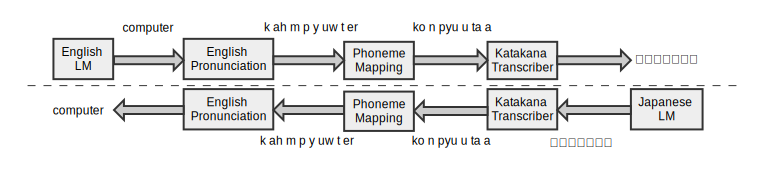
\includegraphics[scale=0.62]{figures/fsts}\tabularnewline
\end{tabular}
\caption{\label{font-table} The transliteration generative story as a cascade of FSTs . Each box represents a transducer. \textbf{Top:} transliteration of the word ``computer'' to Japanese. \textbf{Bottom:} the reverse process. PAT jointly trains the two cascades by maximizing both the data log-likelihood and the parameter agreement of the two (shaded) phoneme mapping models. The blank FSTs are held fixed. }
\label{fig:fsts}
\end{center}
\end{figure*}

Transliteration is a mapping of terms between writing systems of different languages. 
Usually, the mapping tries to preserve the sound of a term as it is uttered in the original language. 
For example, the word ``computer'' in English is transliterated to Japanese as ``ko n pyu u ta a'' (in Romaji\marginpar{Romaji or Katakana?}). 
The process restoring transliterated foreign words to their original script is called \emph{back-transliteration}.

Knight and Graehl \shortcite{KG98} suggest a generative story for the transliteration of an English term $\vw$ into Japanese term $\vk$ (see top of Figure \ref{fig:fsts}): 
\begin{enumerate}
\item First, a word $\vw$ is generated according to an English language model (LM)
$p(\vw)$.
\item $\vw$ is then mapped to an English phonemes sequence $\ve=(\ve_1,\ldots,\ve_I)$ according to a pronunciation model.
\item The phoneme sequence $\ve$ is mapped to a sequence of Japanese phonemes $\vj=(\vj_1,\ldots,\vj_J)$ according to a phoneme mapping model $p(\vj \mid \ve)$.
\item Finally, the Japanese phoneme sequence $\vj$ is mapped to a
Japanese word $\vk$ in Katakana.
\end{enumerate}
Each of their models is encoded as an FST that can be constructed and trained independently. Knight and Graehl estimate FSTs 1,2,4 over monolingual data only, whereas the phoneme mapping model $p(\vj \mid \ve)$ (\eqn{eqn:parallel}) is trained over a parallel phoneme corpus $\set{(\ve_{n},\, \vj_{n})}$ and further restricted such that each English phoneme is allowed to map to either one or two Japanese phonemes only.

However, collecting parallel data is a time consuming, laborious process.
To combat the need for parallel data, Ravi and Knight \shortcite{RK09} suggest to estimate model 2 in the decipherment setting, for which only Japanese words $K=\set{\vk_n}_{n=1}^{|K|}$ need be collected. 
Assuming one-to-one transformations for models 2 and 4 
(so that $p(\vw) = p(\ve)$ and $p(\vk) = p(\vj)$) 
the generative process for transliteration is identical to that of \eqn{eqn:decipherment}:
\begin{align*}
p(\vk)=p(\vj)
=&\sum_\vw p(\vw) \cdot p(\vj \mid \vw)\\
=&\sum_\ve p(\ve) \cdot p(\vj \mid \ve)\\
=&\sum_\ve p(\ve) \sum_\va  p(\va,  \vj \mid \ve)
\end{align*}
Where $\va=((\va_{1}^{\tstart}, \va_{1}^{\tend}),\ldots,(\va_{I}^{\tstart}, \va_{I}^{\tend}))$ denotes a \emph{source-to-target} monotone alignment sequence
under which $\ve_i$ is mapped to one or two phonemes from $\vj$, denoted $\vj[\va_{i}^{\tstart}:\va_{i}^{\tend}]$.
By monotone alignment we mean that $\va_{i}^{\cdot} \le \va_{i+1}^{\cdot}$ and $1 \le \va_{i}^{\tstart} \le \va_{i}^{\tend} \le J$ for all $i$.
The overall probability of this mapping is then:
\begin{equation}
p(\va,  \vj \mid \ve) = \prod_{i=1}^{I} t(\vj[a_{i}^{\tstart}:a_{i}^{\tend}] \mid \ve_{i})
\label{eqn:trans}
\end{equation}
where $t(\vj[a_{i}^\tstart:a_{i}^\tend] \mid \ve_{i})$ denotes the probability of transliterating English phoneme $\ve_i$ to Japanese phoneme(s) $\vj[a_{i}^\tstart:a_{i}^\tend]$.


%Thus, a Japanese phoneme sequence $\vj$ can arise from any English pronunciation sequence $\ve$ that is producible by the language and pronunciation models:
%$$
%p(\vj) = \sum_{\ve} p(\ve)\cdot p(\vj \mid \ve)$$
%As a result, the data log-likelihood takes the form:
%\begin{align}
%L(J)& = \sum_{\mathbf{j}\in J} \log \sum_{\mathbf{e}} \PP(\mathbf{j}\mid \mathbf{e})\cdot \PP(\mathbf{e})
%\end{align}
%Once the model is trained, back-transliteration (decoding) of Japanese words back to English can be done using the Viterbi algorithm.

%We note a few points:
%\begin{itemize}
%\item The computational cost of solving this problem is much higher than the parallel case since we are forced to use the language and pronunciation models during training time. 
%\item Only the phoneme mapping parameters $P(j_{m}\mid e_{m})$ are trained while
%the other FSTs' parameters are kept fixed.
%\end{itemize}









%We briefly discuss two machine translation related tasks - word alignment and phonetic back-transliteration.
%Both tasks share a similar generative story that describes how source sequences $e=(e_1, \ldots, e_I)$ (of strings or phonemes) are distorted (reordered) and translated into target sequences $f = (f_1, \ldots, e_J)$.
%As shall be seen, their sole difference lies in the permitted set of distortions - whereas all alignments are permitted in word alignment, only monotone alignments are allowed in back-transliteration.



%In machine learning, and machine translation in particular, generative stories describes transformations of entities $e$ (strings, phonemes) from a source language to entities $f$ in a target language.
%The generative story explicitly construct conditional probability distributions $P(f\mid e)$ where $e$ is an entity from $L_{E}$ and $f$ is an entity from $L_{F}$.
%The predominant approach for training generative models is the EM
%framework which iteratively maximizes log-likelihood of the observed
%data $X=\{e_{n},\, f_{n}\}_{n=1}^{N}$:
%\begin{align*}
%\max_{P}L(P\mid X)=\max_{P}\sum_{n}\log P(f_{n}\mid e_{n})
%\end{align*}
%In a setting like word alignment where models are trained in both directions, we adopt the notation $\PP(e_{n}\mid f_{n})$ for one direction and $\QQ(f_{n}\mid e_{n})$
%for the other. 
%The two models can be independently trained by maximizing each data log-likelihood function separately:
%\begin{align*}
%\PP^{*} &= \argmax_{\PP}L(\PP\mid X)\\
%\QQ^{*} &= \argmax_{\QQ}L(\QQ\mid X).
%\end{align*}


\section{Parameter Agreement Training}
\label{sec:method}

In this section we propose a method for jointly training two word alignment models, a source-to-target model $\TA$ and a target-to-source model $\TB$, by regularizing their parameters to respect the invertibility of the underlying alignment task. 
We therefore named our method \emph{Model Invertibility Regularization} (MIR).

Specifically, our regularizer operates on the t-tables parameters $\tA, \tB$ of the two models, as defined as follows:
Let matrices $T_1, T_2$ denote the t-tables $\tA, \tB$ in matrix form and consider their multiplication $T=T_1 T_2$. 
The resulting matrix $T$ is a stochastic square matrix of dimension $|V_1|\times|V_1|$ where $|V_1|$ represents the size of the source-language vocabulary.
Each entry $T_{ij}$ represents the total probability mass mapped from source word $e_i$ to source word $e_j$ by first applying the source-to-target mapping $T_1$ and then the target-to-source mapping $T_2$.

In particular, each entry $T_{ii}$ on the diagonal holds the probability of mapping a source entity back onto itself, a quantity we intuitively believe should be high.
We therefore (initially) consider the trace of $T$:
$$Tr[T]=\sum_i T_{ii}=\sum_{e,f}t_{1}(f\mid e)t_{2}(e\mid f)$$
and further note that $Tr[T]=Tr[T_{1}T_{2}]=Tr[T_{2}T_{1}]$ so that the trace just as equally captures how much the target entities map onto themselves.

Now, since $T$ is stochastic, setting $T:=I$ maximizes the trace $Tr[T]$ (where $I$ denotes the identity matrix). In other words, the more $T_1$ and $T_2$ behave as (pseudo-)inverses of each other, the higher the trace would be. This exactly fits with our intuition regarding invertibility.

Unfortunately however, the trace is not concave in both $T_1$ and $T_2$, a property which will become desirable in optimization.
Therefore, we modify the trace regularizer to a similar term:
\begin{equation}
\label{eqn:R}
R(t_{1},t_{2})=\sum_{e,f}\sqrt{t_{1}(f\mid e)t_{2}(e\mid f)}
\end{equation}

Concavity of $R$ in both $t_1, t_2$ follows from the observation that it is a sum of concave functions - each term in the summation is a geometric mean, which is concave in its parameters.

\subsection{Optimization With/Without Parallel Data}

We consider two data scenarios for MIR -
In the parallel data setting, we observe $N$ paired sequences $\set{\vx^n_1}_{n=1}^N=\set{(\ve^n, \vf^n)}_{n=1}^N$ or, equivalently, $\set{\vx^n_2}_{n=1}^N=\set{(\vf^n, \ve^n)}_{n=1}^N$.

In the non-parallel data setting, we observe two sets of data points $\set{\vx^n_1}_{n=1}^{N_1} = \set{\ve^n}_{n=1}^{N_1}$ and $\set{\vx^n_2}_{n=2}^{N_2} = \set{\vf^n}_{n=1}^{N_2}$.

For $k\in\set{1,2}$, the probability of the $n$th sample under the $k$th model $\T_k$ is denoted $\pk(\vx_k^n; \Tk)$.
Specifically, in the parallel data setting, the directional probability of $\vx_k^n$ under its model is:
\begin{align*}
\pA(\vx_1^n; \TA) = p(\vf^n \mid \ve^n; \TA)\\
\pB(\vx_2^n; \TB) = p(\ve^n \mid \vf^n; \TB)
\end{align*}
whereas in the non-parallel data setting, the probability is defined:
\begin{align*}
\pA(\vx_1^n; \TA) = p(\vf^n; \TA)\\
\pB(\vx_2^n; \TB) = p(\ve^n; \TB)
\end{align*}

Similarly to the multi-task learning approach of \newcite{liang+:2006:align} we formulate a single objective function for jointly training the two directional alignment models $\TA, \TB$. 
Our objective function maximizes the regularized log-likelihoods $\{{L_k}\}_{k=1,2}$ of the observed data using our proposed MIR regularizer $R$ (Eq. \ref{eqn:R}):
\begin{equation}
\max_{\TA, \TB}\,\, \lambda R(\TA, \TB)
%+\sum_{k\in\set{1,2}} \log \sum_n \pk(\vx^n; \Tk)
+\sum_{k\in\set{1,2}} L_k(\set{\vx_k^n}; \Tk)
\label{eqn:joint}
\end{equation}
Where $\lambda\ge0$ is a tunable hyperparameter.


%\subsection{remove me}
%In word alignment, it is common practice to train alignment models in both source-to-target and target-to-source directions and then apply symmetrization techniques to the resulting source-to-target and target-to-source alignments. 
%%Alignment symmetrization heuristics, such as intersection, union or grow-diag-final-and play a significant role in reducing alignment errors and ultimately improving translation quality.
%The improvement gained by these post-processing heuristics suggest that each (directional) model suffers from different errors, and that those errors can be mitigated by symmetrization.
%
%Observing this, \newcite{liang+:2006:align} formulate Alignment by Agreement, which maximizes both the observed data-likelihoods as well as a measure of agreement between the two models' posteriors.
%Showing significant reductions in AER, they demonstrate the effectiveness of jointly learning the models. However, because both symmetrization heuristics and Alignment by Agreement try to create agreement between the inferences of the two models, they necessarily run the two models on the same data, which must be parallel.
%
%In this section, we describe Parameter Agreement Training (PAT), a method for jointly learning directional models that does not depend on parallel data. 	
%We follow Liang et al. (2006) in formulating a joint objective function for training the two directional alignment models, but define the agreement measure in a way that can be applied either to the parallel data or non-parallel data setting.
%
%In the parallel data setting, we observe $N$ paired sequences $\set{\vx^n_1}_{n=1}^N=\set{(\ve^n, \vf^n)}_{n=1}^N$ or, equivalently, $\set{\vx^n_2}_{n=1}^N=\set{(\vf^n, \ve^n)}_{n=1}^N$.
%
%In the non-parallel data setting, we observe two sets of data points $\set{\vx^n_1}_{n=1}^{N_1} = \set{\ve^n}_{n=1}^{N_1}$ and $\set{\vx^n_2}_{n=2}^{N_2} = \set{\vf^n}_{n=1}^{N_2}$.
%
%Let $\TA$ and $\TB$ represent the two directional models' parameters.
%For $k\in\set{1,2}$, the probability of the $n$th sample under the $k$th model is denoted $\pk(\vx_k^n; \Tk)$.
%Specifically, in the parallel data setting, the directional probability of $\vx_k^n$ under its model is:
%\begin{align*}
%\pA(\vx_1^n; \TA) = p(\vf^n \mid \ve^n; \TA)\\
%\pB(\vx_2^n; \TB) = p(\ve^n \mid \vf^n; \TB)
%\end{align*}
%whereas in the non-parallel data setting, the probability is defined:
%\begin{align*}
%\pA(\vx_1^n; \TA) = p(\vf^n; \TA)\\
%\pB(\vx_2^n; \TB) = p(\ve^n; \TB)
%\end{align*}
%
%In either case, independently optimizing each model entails the maximization of its data log-likelihood (for $k\in{1,2}$):
%$L_k(\set{\vx^n_k}; \Tk)=\sum_n \log\pk(\vx_k^n; \Tk)$
%%
%%\begin{align*}
%%\max_{\Tk}\,\,L_k(\set{\vx^n_k}; \Tk)= 
%%\max_{\Tk}\,\,  \sum_n \log \pk(\vx_k^n; \Tk)
%%\end{align*}
%
%To jointly optimize the two models, a coupling term $R(\TA, \TB)$ is introduced, which encodes a measure of agreement between the two models.
%The resulting joint optimization problem takes the following form:
%\begin{equation}
%\max_{\TA, \TB}\,\, \lambda R(\TA, \TB)
%%+\sum_{k\in\set{1,2}} \log \sum_n \pk(\vx^n; \Tk)
%+\sum_{k\in\set{1,2}} L_k(\set{\vx_k^n}; \Tk)
%\label{eqn:joint}
%\end{equation}
%with $\lambda\ge0$ being a tunable hyperparameter.
%
%\subsection{Parameter Agreement Measure}
%Both the word alignment and transliteration models presented in Section \ref{sec:background} are parameterized by a translation table.
%Considering these tables in both directions, $t_1$ and $t_2$, we suggest the following parameter agreement measure: 
%\begin{equation}
%R(\TA, \TB) = \sum_{e,f} \sqrt{t_1(f \mid e) \cdot t_2(e \mid f)}
%\label{eqn:R}
%\end{equation}
%where $\ve$ and $\vf$ range over all source and target entity types.
%Note that $R$ disregards the distortion parameters $a$ (if at all present).
%
%Our agreement measure has several appealing properties.
%Using the Cauchy-Schwarz inequality, we can bound $R(\TA, \TB) \le \sqrt{|V_E|\cdot|V_F|}$ where $|V_E|, |V_F|$ denote the source and target vocabulary size.
%%\begin{align*}
%%R(\TA, \TB) 
%%%\sum_{e,f} \sqrt{(t_1(\ve \mid \vf) \cdot t_2(\vf \mid \ve))} 
%%\le &\sqrt{ (\sum_{e,f} t_1(\vf \mid \ve)) (\sum_{e,f} t_2(\ve \mid \vf))}\\
%%= &\sqrt{(|V_E|\cdot|V_F|)}
%%\end{align*}
%In particular, when $|V_E|=|V_F|$, the maximum is attained on parameter configurations for which $t_1(\vf \mid \ve) = t_2(\ve \mid \vf)$ over all entity pairs.
%% demonstrating that this agreement term is not biased towards any particular property (e.g, sparsity).
%Thus, the objective in \eqn{eqn:joint} balances between similarity in parameter magnitude and data likelihood. 
%%\marginpar{\bluetext{TL: this seems like a good place to say something about invertibility}}
%
%Another appealing property of $R$ is its concavity, which follows since $R$ is the sum of concave functions $h(x, y)=\sqrt{xy}$ over a closed convex set (see the concavity proof for $h$ in the appendix).
%
%% TODO: other agreement terms
%
%%We now describe our method, which we call Parameter Agreement Training.
%%In translation, we believe that if a word $e$ can be translated
%%to a word $f$, then $f$ can be translated to~$e$. 
%%This intuition holds for other tasks such as word or phoneme alignment.
%%Thus, a desirable form of model agreement is parameter
%%sparsity agreement: 
%%\begin{align*}
%%P_{0}(f\mid e) = 0 \text{ iff } P_{1}(e\mid f)=0.
%%\end{align*}
%%%A possibly simpler form of agreement is $P_{0}(e\,,f) = P_{1}(f,\: e)$ which encodes
%%% equality in joint distributions.
%
%%\subsection{Regularization}
%%To encourage this form of parameter agreement we add a regularizer that couples the two models together:
%%\begin{align}
%%\max_{\PP\,,\QQ}&\,\,L(\PP | X)+L(\QQ | X)+\lambda R(\PP,\, \QQ)
%%\end{align}
%%where $\lambda\ge0$ is a regularization coefficient to be tuned and
%%\begin{align}
%%R(\PP, \QQ) = \sum_{e,f}\sqrt{\PP(f\mid e)\QQ(e\mid f)} .
%%\end{align}
%%This regularizer has two attractive properties:
%%\begin{itemize}
%%\item It is concave on the probability simplex which lends to an efficiently solvable convex optimization program when the log-likelihood terms are themselves concave.
%
%%Concavity proof: 
%%The regularizer is a sum of concave functions defined over a convex set. 
%%each summand is concave  the region $[0,1]^{2}$ and the sum of concave functions is concave)
%%\item It encourages parameter sparsity agreement - If $\PP(e \mid f) = 0$ but $\QQ(f\mid e) > 0$, shifting weight away from $\QQ(f \mid e)$ could only increase the regularizer value.
%%\end{itemize}
%%In practice, we found the following two regularizers useful:`
%%\begin{align*}
%%R_{GM}(P_{0},\, P_{1}) & =  \sum_{e,f}\sqrt{P_{0}(f\mid e)\cdot P_{1}(e\mid f)}\\
%%%R_{CD}(P_{0},\, P_{1}) & =  -\frac{1}{2}\sum_{e,f}(P_{0}(e\mid f)-P_{1}(f\mid e))^{2}
%%\end{align*}
%%Where \emph{GM }stands for 'geometric mean' and \emph{CD} for 'conditional
%%difference'. 
%%
%%Note that both regularizers are concave on the probability simplex
%%- each term in their summation is concave over the region $[0,1]^{2}$,
%%and the sum of concave functions is concave. One difference between
%%$R_{GM}$ and $R_{CD}$ is that, while both regularizers attain higher
%%values when the conditional distributions agree, $R_{GM}$ attains
%%its maximum when those distributions are sparse (need example?)



\subsection{Optimization Procedure}\label{subsec:optimization}
Using our concave regularizer, MIR optimization (\eqn{eqn:joint}) neatly falls under the EM framework \cite{Dempster:1977} and maintains the convergence properties of the underlying algorithms. 
On a high level, since the MIR regularizer operates only on the model parameters, computation of the E-step can be carried out independently for each model. 
In this sense, MIR is orthogonal to the complexity of the models' inference space.
The additional algorithmic cost incurred by adding the regularizer resides in the M-step, where we now optimize a single (concave) objective function involving both models and the regularizer.

Specifically, In the E-step, each model $\Tk$, $k\in\set{1,2}$ is held fixed and its posterior distribution over the missing data $\vz_k^n$ is computed per each observation, $\vx_k^n$:
\begin{align*}
q_k(\vz\kn, \vx\kn) & \mathrel{:=} \pk(\vz\kn \mid \vx\kn ; \Tk)
%\textbf{parallel data}: q_k(\va \mid \ve, \vf) :=& \pA(\va \mid \ve, \vf; \TA) \\
%\textbf{decipherment}: q_1(\va, \ve \mid \vf) :=& \pA(\va, \ve \mid \vf; \TA)
\end{align*}
where, in the parallel data setting, only the alignment is missing ($\vz\kn = \va\kn$) and in the non-parallel data setting, both the alignment and the origin entity are missing
($\vz_1^n = (\va_1^n, \ve^n), \vz_2^n = (\va_2^n, \vf^n)$).

In the M-step, the computed posteriors are used to define a convex optimization program that maximizes the regularized sum of expected complete-data log-likelihoods:
 %$\TA, \TB$:
\begin{align*}
%(\TA', \TB') 
& \arg\max_{\TA, \TB}
\lambda R(\TA,\TB)\\
&\quad {} + \sum_{k\in\{1,2\}, n} q_k(\vz\kn, \vx\kn) \log p_k(\vx\kn, \vz\kn)
\end{align*}
Where $n$ ranges over the appropriate sample set.

On a more operative level, for models $\Tk$ that can be encoded as wFST (such as the IBM and HMM word alignment models) the E-step posteriors $q_k$ can be computed efficiently and exactly using dynamic programming \cite{Eisner02}. 
More advanced models resort to approximation techniques - for example, the fertility-based word alignment models apply hill-climbing and sampling heuristics in order to efficiently estimate the posteriors [REFERENCE?].

Once the posteriors $q_k$ are computed we derive expected counts $\Ch_1^{e,f} $ and $\Ch_2^{e,f}$, where $\Ch_k^{e,f}$ denotes the expected number of times a source-entity type $e$ is seen aligned to a target-entity type $f$ according to the posteriors $q_k$. These expected counts are then used in constructing the M-step program.

%For the IBM and the HMM word alignment models, the modeling assumptions allow the distortion and the translation parameters to be optimized independently in the M-step. 

Specifically, MIR regularization couples only the t-table parameters and yields the following maximization problem in $t_1, t_2$:
\begin{align}
\arg\max_{t_1, t_2}&\sum_{e,f}  \Ch_1^{e,f}\log t_1(f \mid e) + 
\\
& \sum_{e,f} \Ch_2^{e,f} \log t_2(e \mid f) + 
\lambda R(t_1, t_2) \nonumber
\label{eqn:Mobj}
\end{align}
which can be efficiently solved using convex programming techniques due to the   concavity of $R$ and the complete-data log-likelihoods in both $t_1$ and $t_2$.

In our implementation we used Projected Gradient Descent \cite{bertsekas1999nonlinear} where at each step, the parameters $(t_1, t_2)$ are updated according to the gradient of the M-step objective at $(t_1, t_2)$ and then projected back onto the probability simplex. 
We used simple stopping conditions based on objective function value convergence and a bounded number of iterations.

As for the remaining model parameters (if there are any) - their M-step estimation is left unchanged. In word alignment, this implies the usual closed-form count-and-divide solution for the distortion, fertility and other parameters.


%
%\iffalse
%\subsection{MIR for Word Alignment}
%As described in section~\ref{subsec:optimization}, in the E-step, we compute the posterior distribution over alignments in each direction, which amounts to computing the expected counts  $\E_1[C(e,f)] $ and $\E_2[C(e,f)] $, where $C(e,f)$ is the number of times $e$ is seen aligned to $f$. 
%In the M-step, we use the expected counts to re-estimate model parameters by maximizing the coupled expected complete data log likelihood. 
%In our work, we only encourage agreement between the translation probabilities $t(e \mid f)$ and $t(f \mid e)$. 
%Thus, the M-step objective function with respect to the translation probabilities is:
%\begin{align*}
%&\sum_{e,f}  \E_1[C(e,f)] \log t(e \mid f)  + {}\\ 
%&\quad \E_2[C(e,f)] \log t(f \mid e) + \sqrt{t(e \mid f)t(f \mid e)}, 
%\end{align*}
%which is maximized with projected gradient descent. 
%
%The estimation of the distortion probabilities is thus left unchanged (count and divide). We leave PAT of the distortion parameters for future work. 
%\fi


%At each time step, the models $\PP, \QQ$ are updated according to the gradient of the regularized objective function 
%%$\frac{\partial}{\partial \PP}(L(\PP \mid X)+\lambda R(\PP, \QQ)$
%and projected back onto the probability simplex. 
%
%Inspecting the regularizer's gradient we see that each update brings the two models closer:
%\begin{align*}
%\frac{\partial R}{\partial t_1(\vf\mid\ve)}
%&=\sqrt{\frac{t_2(\ve\mid\vf)}{2 t_1(\vf\mid\ve)}} \\
%\frac{\partial R}{\partial t_2(\ve\mid\vf)}
%&=\sqrt{\frac{t_1(\vf\mid\ve)}{2 t_2(\ve\mid\vf)}}
%\end{align*}
%%
%With symmetric terms for the gradient in $\QQ$. Note that the square root is taken entry-wise.


%\subsection{Agreement Training}
%In word alignment, it is common practice to train alignment models in both source-to-target and target-to-source directions and then apply symmetrization techniques to the resulting source-to-target and target-to-source alignments. 
%%Alignment symmetrization heuristics, such as intersection, union or grow-diag-final-and play a significant role in reducing alignment errors and ultimately improving translation quality.
%The improvement gained by these post-processing heuristics suggest that each (directional) model suffers from different errors, and that those errors can be mitigated by symmetrization.
%
%Observing this, \newcite{liang+:2006:align} formulate Alignment by Agreement, which maximizes both the observed data-likelihoods as well as a measure of agreement between the two models' posteriors.
%Showing significant reductions in AER, they demonstrate the effectiveness of jointly learning the models. However, because both symmetrization heuristics and Alignment by Agreement try to create agreement between the inferences of the two models, they necessarily run the two models on the same data, which must be parallel.
%
%In this section, we describe Parameter Agreement Training (PAT), a method for jointly learning directional models that does not depend on parallel data. 	
%We follow Liang et al. (2006) in formulating a joint objective function for training the two directional alignment models, but define the agreement measure in a way that can be applied either to the parallel data or non-parallel data setting.
%
%In the parallel data setting, we observe $N$ paired sequences $\set{\vx^n_1}_{n=1}^N=\set{(\ve^n, \vf^n)}_{n=1}^N$ or, equivalently, $\set{\vx^n_2}_{n=1}^N=\set{(\vf^n, \ve^n)}_{n=1}^N$.
%
%In the non-parallel data setting, we observe two sets of data points $\set{\vx^n_1}_{n=1}^{N_1} = \set{\ve^n}_{n=1}^{N_1}$ and $\set{\vx^n_2}_{n=2}^{N_2} = \set{\vf^n}_{n=1}^{N_2}$.
%
%Let $\TA$ and $\TB$ represent the two directional models' parameters.
%For $k\in\set{1,2}$, the probability of the $n$th sample under the $k$th model is denoted $\pk(\vx_k^n; \Tk)$.
%Specifically, in the parallel data setting, the directional probability of $\vx_k^n$ under its model is:
%\begin{align*}
%\pA(\vx_1^n; \TA) = p(\vf^n \mid \ve^n; \TA)\\
%\pB(\vx_2^n; \TB) = p(\ve^n \mid \vf^n; \TB)
%\end{align*}
%whereas in the non-parallel data setting, the probability is defined:
%\begin{align*}
%\pA(\vx_1^n; \TA) = p(\vf^n; \TA)\\
%\pB(\vx_2^n; \TB) = p(\ve^n; \TB)
%\end{align*}
%
%In either case, independently optimizing each model entails the maximization of its data log-likelihood (for $k\in{1,2}$):
%$L_k(\set{\vx^n_k}; \Tk)=\sum_n \log\pk(\vx_k^n; \Tk)$
%%
%%\begin{align*}
%%\max_{\Tk}\,\,L_k(\set{\vx^n_k}; \Tk)= 
%%\max_{\Tk}\,\,  \sum_n \log \pk(\vx_k^n; \Tk)
%%\end{align*}
%
%To jointly optimize the two models, a coupling term $R(\TA, \TB)$ is introduced, which encodes a measure of agreement between the two models.
%The resulting joint optimization problem takes the following form:
%\begin{equation}
%\max_{\TA, \TB}\,\, \lambda R(\TA, \TB)
%%+\sum_{k\in\set{1,2}} \log \sum_n \pk(\vx^n; \Tk)
%+\sum_{k\in\set{1,2}} L_k(\set{\vx_k^n}; \Tk)
%\label{eqn:joint}
%\end{equation}
%with $\lambda\ge0$ being a tunable hyperparameter.
%
%\subsection{Parameter Agreement Measure}
%Both the word alignment and transliteration models presented in Section \ref{sec:background} are parameterized by a translation table.
%Considering these tables in both directions, $t_1$ and $t_2$, we suggest the following parameter agreement measure: 
%\begin{equation}
%R(\TA, \TB) = \sum_{e,f} \sqrt{t_1(f \mid e) \cdot t_2(e \mid f)}
%\label{eqn:R}
%\end{equation}
%where $\ve$ and $\vf$ range over all source and target entity types.
%Note that $R$ disregards the distortion parameters $a$ (if at all present).
%
%Our agreement measure has several appealing properties.
%Using the Cauchy-Schwarz inequality, we can bound $R(\TA, \TB) \le \sqrt{|V_E|\cdot|V_F|}$ where $|V_E|, |V_F|$ denote the source and target vocabulary size.
%%\begin{align*}
%%R(\TA, \TB) 
%%%\sum_{e,f} \sqrt{(t_1(\ve \mid \vf) \cdot t_2(\vf \mid \ve))} 
%%\le &\sqrt{ (\sum_{e,f} t_1(\vf \mid \ve)) (\sum_{e,f} t_2(\ve \mid \vf))}\\
%%= &\sqrt{(|V_E|\cdot|V_F|)}
%%\end{align*}
%In particular, when $|V_E|=|V_F|$, the maximum is attained on parameter configurations for which $t_1(\vf \mid \ve) = t_2(\ve \mid \vf)$ over all entity pairs.
%% demonstrating that this agreement term is not biased towards any particular property (e.g, sparsity).
%Thus, the objective in \eqn{eqn:joint} balances between similarity in parameter magnitude and data likelihood. 
%%\marginpar{\bluetext{TL: this seems like a good place to say something about invertibility}}
%
%Another appealing property of $R$ is its concavity, which follows since $R$ is the sum of concave functions $h(x, y)=\sqrt{xy}$ over a closed convex set (see the concavity proof for $h$ in the appendix).
%
%% TODO: other agreement terms
%
%%We now describe our method, which we call Parameter Agreement Training.
%%In translation, we believe that if a word $e$ can be translated
%%to a word $f$, then $f$ can be translated to~$e$. 
%%This intuition holds for other tasks such as word or phoneme alignment.
%%Thus, a desirable form of model agreement is parameter
%%sparsity agreement: 
%%\begin{align*}
%%P_{0}(f\mid e) = 0 \text{ iff } P_{1}(e\mid f)=0.
%%\end{align*}
%%%A possibly simpler form of agreement is $P_{0}(e\,,f) = P_{1}(f,\: e)$ which encodes
%%% equality in joint distributions.
%
%%\subsection{Regularization}
%%To encourage this form of parameter agreement we add a regularizer that couples the two models together:
%%\begin{align}
%%\max_{\PP\,,\QQ}&\,\,L(\PP | X)+L(\QQ | X)+\lambda R(\PP,\, \QQ)
%%\end{align}
%%where $\lambda\ge0$ is a regularization coefficient to be tuned and
%%\begin{align}
%%R(\PP, \QQ) = \sum_{e,f}\sqrt{\PP(f\mid e)\QQ(e\mid f)} .
%%\end{align}
%%This regularizer has two attractive properties:
%%\begin{itemize}
%%\item It is concave on the probability simplex which lends to an efficiently solvable convex optimization program when the log-likelihood terms are themselves concave.
%
%%Concavity proof: 
%%The regularizer is a sum of concave functions defined over a convex set. 
%%each summand is concave  the region $[0,1]^{2}$ and the sum of concave functions is concave)
%%\item It encourages parameter sparsity agreement - If $\PP(e \mid f) = 0$ but $\QQ(f\mid e) > 0$, shifting weight away from $\QQ(f \mid e)$ could only increase the regularizer value.
%%\end{itemize}
%%In practice, we found the following two regularizers useful:`
%%\begin{align*}
%%R_{GM}(P_{0},\, P_{1}) & =  \sum_{e,f}\sqrt{P_{0}(f\mid e)\cdot P_{1}(e\mid f)}\\
%%%R_{CD}(P_{0},\, P_{1}) & =  -\frac{1}{2}\sum_{e,f}(P_{0}(e\mid f)-P_{1}(f\mid e))^{2}
%%\end{align*}
%%Where \emph{GM }stands for 'geometric mean' and \emph{CD} for 'conditional
%%difference'. 
%%
%%Note that both regularizers are concave on the probability simplex
%%- each term in their summation is concave over the region $[0,1]^{2}$,
%%and the sum of concave functions is concave. One difference between
%%$R_{GM}$ and $R_{CD}$ is that, while both regularizers attain higher
%%values when the conditional distributions agree, $R_{GM}$ attains
%%its maximum when those distributions are sparse (need example?)
%
%\subsection{Optimization Procedure}\label{subsec:optimization}
%Using a concave agreement measure, the optimization of \eqn{eqn:joint} neatly falls under the EM framework \cite{Dempster:1977}.
%
%In the E-step, each model $\Tk$, $k\in\set{1,2}$ is held fixed and its posterior distribution over the missing data $\vz_k^n$ is computed per each observation $\vx_k^n$:
%\begin{align*}
%q_k(\vz\kn, \vx\kn) & \mathrel{:=} \pk(\vz\kn \mid \vx\kn ; \Tk)
%%\textbf{parallel data}: q_k(\va \mid \ve, \vf) :=& \pA(\va \mid \ve, \vf; \TA) \\
%%\textbf{decipherment}: q_1(\va, \ve \mid \vf) :=& \pA(\va, \ve \mid \vf; \TA)
%\end{align*}
%where, in the parallel data setting, only the alignment is missing ($\vz\kn = \va\kn$) and in the non-parallel data setting, both the alignment and the origin entity are missing
%($\vz_1^n = (\va_1^n, \ve^n), \vz_2^n = (\va_2^n, \vf^n)$).
%
%Both the word alignment and transliteration models considered in this paper can be encoded as wFST instances. This implies that the E-step posteriors $q_k$ can be efficiently computed using dynamic programming \cite{Eisner02}. Specifically, for the alignment and transliteration models, this amounts to computing the expected counts  $\E_1[C(e,f)] $ and $\E_2[C(e,f)] $, where $C(e,f)$ is the number of times $e$ is seen aligned to $f$ in a alignment sequence. 
%
%In the M-step, the computed posteriors are used to construct the coupled sum of expected complete data log-likelihoods. The resulting expression is maximized with respect to the model parameters:
% %$\TA, \TB$:
%\begin{align*}
%(\TA', \TB') & \mathrel{:=} \arg\max_{\TA, \TB}
%\lambda R(\TA,\TB)\\
%&\quad {} + \sum_{k, n} q_k(\vz\kn, \vx\kn) \log p_k(\vx\kn, \vz\kn)
%\end{align*}
%with $k\in\set{1,2}$ and $n$ ranging over the appropriate set of samples. For the IBM and the HMM word alignment models, the modeling assumptions allow the distortion and the translation parameters to be optimized independently in the M-step. Applying the parameter agreement measure to the translation probabilities (Equation~\ref{eqn:R}), the above objective function can be defined for $t_1(f \mid e)$ and $t_2(e \mid f)$ as:
%\begin{align*}
%&\sum_{e,f}  \E_1[C(e,f)] \log t_1(f \mid e)  + {}\\ 
%&\quad \E_2[C(e,f)] \log t_2(e \mid f) + \sqrt{t_1(f \mid e)t_2(e \mid f)}
%\end{align*}
%
%\noindent
%where the expected counts were computed in the E-step. This objective function applies for the $t_1(f \mid e)$ and $t_2(e \mid f)$ parameters in transliteration as well. Since we only encourage agreement between $t_1$ and $t_2$, the estimation of the distortion probabilities is left unchanged. We leave agreement training of the distortion parameters for future work. 
%
%Owing to the concavity of both $R$ and the data log-likelihood functions, this maximization problem can be efficiently solved using convex programming techniques. 
%We use projected gradient descent \cite{bertsekas1999nonlinear} where at each step, the current $(\TA, \TB)$ parameters are updated according to the gradient of the M-step objective and then projected back onto the probability simplex. We used simple stopping conditions based on objective function convergence or a limited number of iterations.
%
%\iffalse
%\subsection{PAT for Word Alignment}
%As described in section~\ref{subsec:optimization}, in the E-step, we compute the posterior distribution over alignments in each direction, which amounts to computing the expected counts  $\E_1[C(e,f)] $ and $\E_2[C(e,f)] $, where $C(e,f)$ is the number of times $e$ is seen aligned to $f$. 
%In the M-step, we use the expected counts to re-estimate model parameters by maximizing the coupled expected complete data log likelihood. 
%In our work, we only encourage agreement between the translation probabilities $t(e \mid f)$ and $t(f \mid e)$. 
%Thus, the M-step objective function with respect to the translation probabilities is:
%\begin{align*}
%&\sum_{e,f}  \E_1[C(e,f)] \log t(e \mid f)  + {}\\ 
%&\quad \E_2[C(e,f)] \log t(f \mid e) + \sqrt{t(e \mid f)t(f \mid e)}, 
%\end{align*}
%which is maximized with projected gradient descent. 
%
%The estimation of the distortion probabilities is thus left unchanged (count and divide). We leave PAT of the distortion parameters for future work. 
%\fi
%
%
%%At each time step, the models $\PP, \QQ$ are updated according to the gradient of the regularized objective function 
%%%$\frac{\partial}{\partial \PP}(L(\PP \mid X)+\lambda R(\PP, \QQ)$
%%and projected back onto the probability simplex. 
%%
%%Inspecting the regularizer's gradient we see that each update brings the two models closer:
%%\begin{align*}
%%\frac{\partial R}{\partial t_1(\vf\mid\ve)}
%%&=\sqrt{\frac{t_2(\ve\mid\vf)}{2 t_1(\vf\mid\ve)}} \\
%%\frac{\partial R}{\partial t_2(\ve\mid\vf)}
%%&=\sqrt{\frac{t_1(\vf\mid\ve)}{2 t_2(\ve\mid\vf)}}
%%\end{align*}
%%%
%%With symmetric terms for the gradient in $\QQ$. Note that the square root is taken entry-wise.


\section{Deciphering Transliteration}
\label{sec:transliteration}
%In this section we show that PAT leads to better transliteration models even without parallel data.
%
%\subsection{Generative Story}


%\subsection{Parameter Agreement Training}
%In PAT, the model corresponding to the inverse generative story is also used.
%This inverse process is illustrated at the bottom of Figure \ref{fig:fsts}.
%
%The training data for the reverse direction consists of set of English pronunciations  $E=\{\mathbf{e_n}\}_{n=1}^{|E|}$ and independent training maximizes:
%\begin{align}
%L(E)& = \sum_{\mathbf{e}\in E} \log \sum_{\mathbf{j}} \QQ(\mathbf{e}\mid \mathbf{j})\cdot \QQ(j)
%\end{align}
%To apply PAT, we maximize the joint regularized objective function:
%\begin{align}
%L(J) + L(E) + \lambda R(\PP(\mathbf{j}|\mathbf{e}), \QQ(\mathbf{e}|\mathbf{j}))
%\label{eqn:dec_obj}
%\end{align}
%Once the two models are trained, Japanese words can be decoded using either model. 
%In practice we followed Ravi and Knight and used the $\PP$.
%\begin{figure*}[t]
%\begin{center}
%\begin{tabular}{ccc}
% &  & \tabularnewline
% & 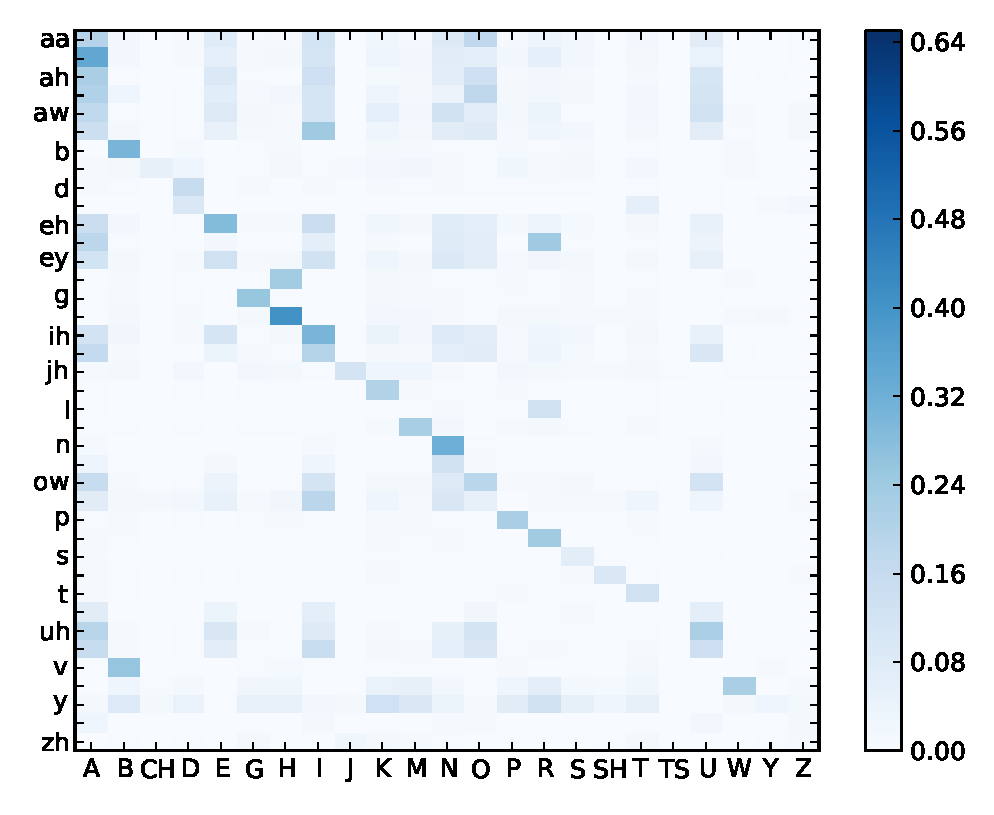
\includegraphics[scale=0.4]{figures/model_11_vanilla} &
% \includegraphics[scale=0.4]{figures/model_11_gm}\tabularnewline
% &  & \tabularnewline
%\end{tabular}
%\caption{Compared to independent training. PAT (right) learns sparser, peaked models.}
%\label{fig:mapping}
%\end{center}
%\end{figure*}

%\begin{figure*}
%\begin{center}
%\begin{tabular}{c}
%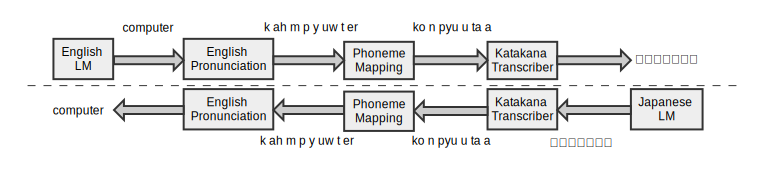
\includegraphics[scale=0.62]{figures/fsts}\tabularnewline
%\end{tabular}
%\caption{\label{font-table} The transliteration generative story as a cascade of FSTs . Each box represents a transducer. \textbf{Top:} transliteration of the word ``computer'' to Japanese. \textbf{Bottom:} the reverse process. PAT jointly trains the two cascades by maximizing both the data log-likelihood and the parameter agreement of the two (shaded) phoneme mapping models. The blank FSTs are held fixed. }
%\label{fig:fsts}
%\end{center}
%\end{figure*}

In this section we present our experiments on deciphering transliterations.
We first reproduced the English-to-Japanese transliteration pipeline of \newcite{RK09} (as described in Section \ref{sec:background} and depicted at the top of Figure \ref{fig:fsts}) and tried to match their reported results.\footnote{Unfortunately, we were unable to obtain all their FSTs and data.}
We then constructed the reverse Japanese-to-English pipeline, required for PAT, and compared the two approaches.

\subsection{The Baseline Decipherment Model}
To reproduce the English-to-Japanese pipeline, we constructed the following FST models:
\begin{enumerate}
\item A unigram language model (LM) of English terms, estimated over the top 40K most frequent capitalized words found in the Gigaword corpus (without smoothing).
\item An English pronunciation FST from the CMU pronunciation dictionary (REFERENCE?).
%http://svn.code.sf.net/p/cmusphinx/code/trunk/cmudict
\item A English-to-Japanese phoneme mapping FST that encodes the phoneme transliteration table $t_1$ (see \eqn{eqn:trans}), constructed based on the best setting reported by \newcite{RK09}. 
We note that $t_1$ is restricted to either 1-to-1 or 1-to-2 phoneme mappings, maintaining consonant parity. See further details in their paper.
\item A hand-built Japanese pronunciation to Katakana FST \cite{RK09}.
\end{enumerate}

\newcite{RK09} report back-transliteration whole-name error rates (WNER) on a list of 100 transliterated US senator names. (In WNER, a decoding is correct if both the first and last name are correctly decoded.)
They train the FST cascade in both parallel and decipherment settings, obtaining 40\% WNER in the parallel setting (trained over 3.3K word pairs) and 73\% WNER on their best decipherment setting (trained over 9.5K Japanese words only).

\subsection{The Inverse Model}
PAT requires a pipeline in the reverse direction, for transliteration of Japanese to English.
% - a Japanese-to-English transliteration pipeline with similar FST models.
We constructed a unigram LM of Katakana terms over the top 25K most frequent Katakana words found in the Japanese news 2005-2008 Leipzig corpora (REFERENCE).
%(http://corpora.informatik.uni-leipzig.de/download.html)

The remaining required FSTs were obtained by inverting the baseline FSTs (that is, FSTs 2,3,4), and the cascade was composed accordingly (depicted at the bottom of Figure \ref{fig:fsts}).
In particular, by inverting $t_1$, we obtained a Japanese-to-English FST $t_2$ that allows only 2-to-1 or 1-to-1 phoneme mappings.

\subsection{Training and Decoding}
For training data, we took the top 50\% most frequent terms from each LM, resulting in a set of 20K English terms and a set of 22.5K Japanese terms.
Using the whole set of terms led to poor baseline results, probably since uncommon English terms are not transliterated, and uncommon Katakana terms may be borrowed from languages other than English.
In any case, it is important to note that the two resulting sets of words are far from being parallel, since they were collected over non-parallel corpora.

Vanilla EM training of the baseline was done using the Carmel finite-state toolkit \cite{graehl97}.
The LM and pronunciation models were held fixed while the parameters of the phoneme mapping model $t_1$ were optimized to maximize the likelihood of the observed set of Japanese terms.

The PAT objective (\eqn{eqn:joint}) was maximized with respect to the phoneme mapping models $(\TA, \TB) = (t_1, t_2)$, with coefficient $\lambda\in\{1,2,3,4\}$.
We manipulated Carmel to compute a single E-step and output the posteriors which we then used to formulate the M-step objective. 
The M-step was solved using our own PGD implementation.\footnote{This implementation is a general purpose PGD solver for convex functions over convex closed sets, and will be released as open-source software.}

To compare against the ordinary parallel data setting, we trained the English-to-Japanese phoneme mapping model $t_1$ with Carmel. We used 4.2K pairs of English and Japanese phoneme sequences. For all models, training was limited to 15 EM iterations.

Finally, back-transliterations of Japanese terms were computed using regular Viterbi decoding of the term with the $t_1$ model only.
Note that symmetrization heuristics are not applicable, since in decipherment we have no parallel data.

\subsection{Results}
\begin{figure*}[t]
\begin{center}
\begin{tabular}{cc}
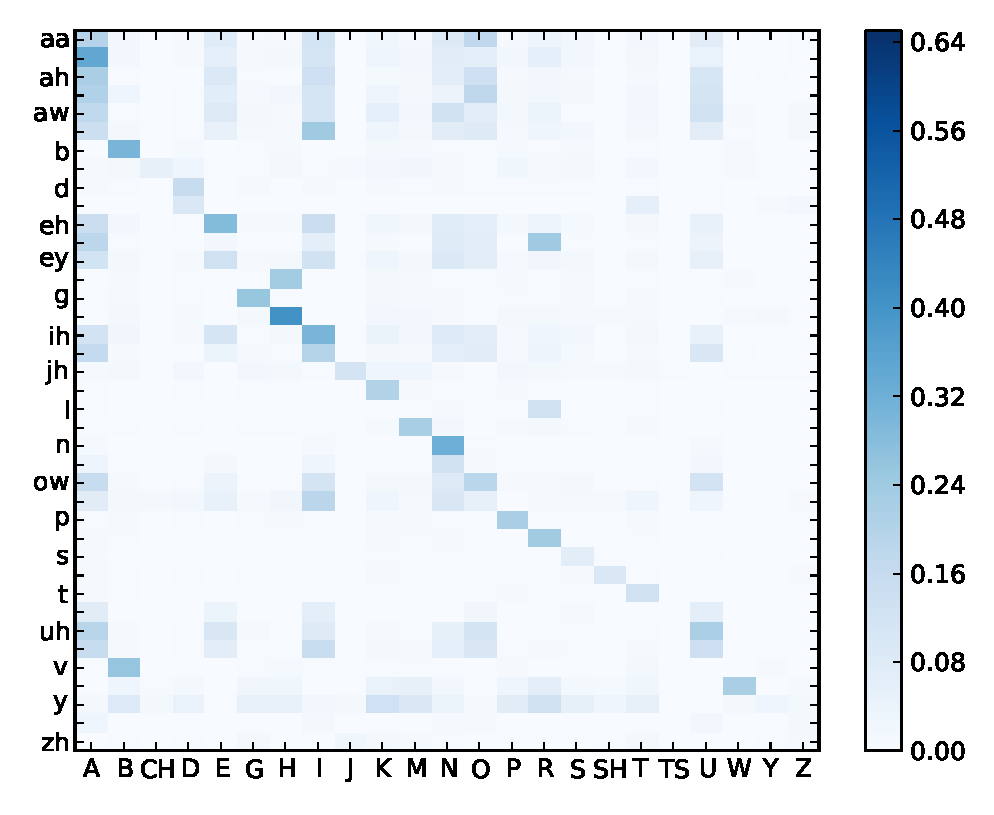
\includegraphics[scale=0.4]{figures/model_11_vanilla} & \includegraphics[scale=0.4]{figures/model_11_gm}\end{tabular}
\end{center}
\caption{The 1-to-1 mapping submatrix of the $t_1$ transliteration table. \textbf{Left}: Independent training. \textbf{Right}: our method (PAT), which learns sparser, peaked models.}
\label{fig:mapping}
\end{figure*}
We compiled our own list of 100 US senator names (first and last) to be used as a test set. 
To tune $\lambda$ we used a development set consisting of 50 frequent Japanese terms and their English origin.

For each method, we selected the $t_1$ model that minimized the development back-transliteration error rate over the 15 iterations, $\lambda$ and the so-called stretch-factor 
$\alpha \in \{1,2,3\}$ that exponentiated the model parameters before decoding (see \newcite{RK09}).

%Table \ref{tbl:transliteration}  %% ref not working for some reason
Table 1
reports WNER, average normalized edit distance (NED) and the number of $t_1$ parameters with value greater than 0.01 ($t_1>0.01$) as an indication of model sparsity. 
Figure \ref{fig:mapping} further compares a portion of the best phoneme mapping table learned by the baseline vs. that learned by PAT, depicting the difference in parameter sparsity.

\begin{table}[h]
\begin{center}
\begin{tabular}{l|c|c|c}
\multicolumn{1}{c|}{} & WNER & NED & $t_1> 0.01$\tabularnewline
\hline 
Independent & 67\% & 23.2 & 649\tabularnewline
PAT & 59\% & 17.3 & 421\tabularnewline
Parallel Data & 43\% & 10.8 & 152\tabularnewline
\end{tabular}

\caption{PAT reduces error rates (WNER, NED) and learns sparser models (number of $t_1$ parameters greater than 0.01).}
\end{center}
\end{table}

Using PAT we were able to significantly reduce the error rate, reducing the gap in WNER between independent and parallel-data settings by 33\% and the gap in NED by nearly half.
This error reduction clearly demonstrates the efficacy of jointly training these models, and of the PAT formulation in particular.





\section{Word Alignment}
\label{sec:alignment}
%Given a \emph{target} French sentence, $\mathbf{f_{1}^{J}} =  f_{1}, f_{2}, \ldots , f_{j}, \ldots, f_{J}$, and a \emph{source} English sentence, $\mathbf{e_{1}^{I}} =  e_{1}, e_{2}, \ldots , e_{i}, \ldots, e_{I}$, word alignment models describe the generative process by which the source sentence creates the target ($E \rightarrow F$) ausing latent alignments $\mathbf{a_{1}^{J}} = a_{1}, a_{2}, \ldots , a_{j}, \ldots, a_{J}$. The alignment variable $a_{j}$ specifies the English word $e_{a_{j}}$ that the French word $f_j$ is aligned to. 
%
%The IBM Models 1--2 and the HMM alignment models have two sets of parameters, the translation probabilities $P_{t}(f_{j} \mid e_{a_{j}})$ and distortion probabilities, $P_{d}(a_{j}\mid a_{j-1},j)$. These models differ in their implementation and estimation of the distortion probabilities, but share the same translation probabilities. The general form of the joint probability  of a target sentence and alignment given the source sentence is:
%
%\begin{equation} \label{eq:joint-prob-align}
%P(\mathbf{f_{1}^{J}}, \mathbf{a_{1}^{J}} \mid \mathbf{e_{1}^{I}})  = \prod_{j=1}^{J} P_{d}(a_{j}\mid a_{j-1},j) P_{t}(f_{j} \mid e_{a_{j}})
%\end{equation}
%
%During training, we typically estimate the parameters that maximize 
%\begin{equation}
%\log \sum_{a_{1}^{J}}  P(\mathbf{f_{1}^{J}}, \mathbf{a_{1}^{J}} \mid \mathbf{e_{1}^{I}}) = \log P(\mathbf{f_{1}^{J}} \mid \mathbf{e_{1}^{I}})
%\end{equation}.
%
%For details on parameter estimation of these models, and how to deal with empty words, the reader can refer to ~\newcite{och+ney:2003}. For translation, we use the \emph{Viterbi} alignments, 
%\begin{equation}
%\hat{\mathbf{a_{1}^{J}}} = \argmax_{\mathbf{a_{1}^{J}}} P(\mathbf{f_{1}^{J}}, \mathbf{a_{1}^{J}} \mid \mathbf{e_{1}^{I}})
%\end{equation}
%The generative story allows each target word $f_{j}$ to align to only one source word $e_{a_j}$. This can be problematic when the target language has compound words that must align to two or more source language words. The standard solution is to train another model in the \emph{reverse} direction ($F \rightarrow E$), $P(\mathbf{e_{1}^{L}}, \mathbf{a_{1}^{L}} \mid \mathbf{f_{1}^{J}})$ and then symmetrize the Viterbi alignments in both directions using heuristics like \emph{grow-diag-final}  ~\cite{koehn+:2003}. Symmetrization remedies some of the mistakes that the independently trained models make, garbage collection in particular ~\cite{liang+:2006:align}. However, the $E \rightarrow F$ and  $F \rightarrow E$ models do not communicate during training, which could guide the parameters in the wrong direction. In ~\newcite{liang+:2006:align} and ~\newcite{ganchev2010posterior}, the authors show that training the alignment models jointly can improve alignment quality. In ~\newcite{liang+:2006:align}, the authors encourage the probabilities over alignments in each direction to agree, per sentence pair. However, this renders the inference intractable and the authors have to resort to an approximation, without specifying the objective that the approximate procedure ends up optimizing. In contrast, we optimize a clear objective which improves in every iteration. In ~\newcite{ganchev2010posterior}, the authors optimize a clear objective which encourages agreement between the alignments. However, their optimization procedure is expensive and scaling to large datasets is a challenge. \marginpar{need to make sure that it doesn't scale. I suspect it doesn't}.
%
%
%\begin{table}[h]
%\begin{center}
%\begin{tabular}{|c|c|c|c|}
%\cline{2-4} 
%\multicolumn{1}{c|}{} & de-en & cz-en & $\PP > 0.01$\tabularnewline
%\hline 
%~\newcite{liang+:2006:align}  & $71$\% & $70$\%  & -\tabularnewline
%\hline 
%PAT (our) & $71$\% & $69$\%  & -\tabularnewline
%\hline 
%\end{tabular}
%\label{tbl:Alignment Results}
%\caption{Alignment F-score improves.}
%\end{center}
%\end{table}

To test the effectiveness of parameter agreement training, we carried out Czech to English and Chinese to English translation experiments, comparing standard EM training, ABA training, and PAT. 

\subsection{Training}
Following standard practice, we first trained our word alignment models on the following parallel data:
\begin{itemize}
\item \textbf{Chinese-English}: selected data from the constrained task of the NIST 2009 Open MT Evaluation.
\item \textbf{Czech-English}: selected data from the Czech-English News Commentary corpus.
\end{itemize} 

For both ABA and vanilla EM training, we used the publicly available word alignment toolkits that implement them. GIZA++, the popular word alignment toolkit\footnote{https://code.google.com/p/giza-pp/}, implements EM training of the IBM and HMM alignment models, and the toolkit for for ABA \footnote{http://cs.stanford.edu/~pliang/software/cross-em-aligner-1.3.zip} trains IBM Model~1 and the HMM word alignment model. For both our baseline approaches, we ran two sets of experiments, one with $5$ iterations of Model~1 followed by  $5$ iterations of the HMM alignment model, and another with $10$ iterations of each. We trained word alignment models in both directions for both language pairs, and symmetrized our alignments with \emph{posterior decoding}, as described in \newcite{liang+:2006:align}. We will go over the details of posterior decoding in Section~\ref{sec:pos-decoding}.

\subsubsection{Parameter Agreement Training For Word Alignment}

As described in section~\ref{subsec:optimization}, in the E-step, we compute expected counts separately from the alignment models in each direction. Specifically, letting $\Theta_{1} = \Theta_{f \rightarrow e}$, and $\Theta_{2} = \Theta_{\mathbf{e} \rightarrow f}$, where $\rightarrow$ indicates the direction of generation in the word alignment generative story, we compute $E_{e \rightarrow f }[C(e,f)] $ and $E_{f \rightarrow e }[C(e,f)] $

\subsection{Posterior Decoding} \label{sec:pos-decoding}


\begin{table*}
\begin{center} \small
\renewcommand{\arraystretch}{1.1}
\begin{tabular}{cc|c|l|l|l|lll}
task & data (M) & system & align F1 (\%)  &\multicolumn{3}{c}{\bleu (\%)} \\
     &      &        &             & 2008 & 2009 & 2010 \\
\hline
\multirow{3}{*}{Chi-Eng} & \multirow{3}{*}{5.3+6.6} & baseline & 64.6  &  23.6 & & \\
        &       & PAT &  70.0 (+5.4) & 24.0 (+0.4) & &  \\
        &       & ABA  & 70.8 (+6.2)& 24.4 (+0.8) & \\
        &       & ABA+PAT  &    & 25.1 (+1.5) & \\
\hline
\multirow{3}{*}{Cze-Eng} & \multirow{3}{*}{1.6+1.8} & baseline & 65.0 & & 16.7 & 17.1  \\
        &       & PAT   & 69.6 (+4.6)& & 17.1 (+0.4)& 17.6 (+0.5)& \\
        &       & ABA    & 70.4 (+5.4) & & 17.1 (+0.4)&  17.7  (+0.6) &\\
        &       & ABA+PAT   &  & &  17.4 (+0.7)& 17.9 (+0.8)&
\end{tabular}
\end{center}
\caption{For Czech-English, the year refers to the WMT shared task; for all other language pairs, the year refers to the NIST Open MT Evaluation.}
\label{tab:results}
\end{table*}



\section{Related Work}
From a general machine learning perspective, our proposed method can be classified as an unsupervised regularized multi-task learning technique \cite{Evgeniou04,Caruana97}.

Our joint objective (\eqn{eqn:joint}) is inspired by ABA \cite{liang+:2006:align}, which suggests a joint optimization problem for training both directional models. 
The proposed agreement measure
$\sum_\vx \log \sum_{\vz} p_1(\vz \mid \vx; \TA) p_2(\vz \mid \vx; \TB)$
requires access to the posteriors of each sample ($\vx=(\ve, \vf)$) under \emph{both} models.
It is this dependency on parallel data that limits the applicability of the ABA formulation to the parallel data setting.
Therefore, in some sense, our work can be viewed as a generalization of \newcite{liang+:2006:align} beyond the parallel data setting.

Current decipherment work seems to focus on large scale MT experiments \cite{Ravi11,Dou13}. 
We believe our approach would be beneficial in those settings as well.

Bi-directional Conversion Between Graphemes and Phonemes Using a Joint N-gram Model. \bluetext{TL: This paper discusses a \textbf{joint} grapheme-to-phoneme model, trained on parallel data -- It may be out of scope.}








\section{Conclusion}
We presented Parameter Agreement Training (PAT) - an unsupervised method for jointly training two bidirectional alignment models that encourages agreement on parameter magnitude and does not depend on the availability of parallel data.

Our formulation is based on the simply observation that the entity translation tables of bi-directional models should maintain a soft notion of invertibility. That is the reverse translation of the translation of an entity is itself.

We developed an efficient, theoretically sound optimization algorithm that falls under the EM framework. We demonstrated our algorithm's effectiveness on two alignment tasks, matching state-of-the-art BLEU scores on the word alignment task (with parallel data), and gaining substantial error reductions in the English-to-Japanese back-transliteration decipherment task.

%We have presented Parameter Agreement Training (PAT) - an approach for jointly training two conditional models that encourages agreement on parameter values.
%We derived an optimization procedure based on the EM framework, and argued that it is efficiently solvable due to the concavity of our agreement regularizer.
%In contrast to previous work on agreement training, we have demonstrated that our approach can be successfully applied even without parallel data.
\bibliographystyle{acl}
\bibliography{thesis}

\end{document}

%%%% old content of abstract / introduction
%	\iffalse
%% this doesn't make a lot of sense
%We present a simple approach that encourages jointly trained conditional models to agree on their parameter values. In contrast to methods that encourage agreement on inferences, our method can be applied in a wider range of settings.
%We demonstrate that our method, called parameter agreement training, leads to state-of-the-art accuracies on word alignment, and significantly improves accuracy on back-transliteration with no parallel data -- almost halving the difference between the previous best method and using parallel data.

%Alignment is a crucial subtask for many larger NLP problems: Word alignments are the backbone for extracting translation rules used in statistical machine translation; phoneme alignments are used to transliterate Japanese katakana to English and vice-versa. The goal is to align entities, which could be words or phonemes, between two sequences, which could be pairs of source and target sentences or pairs of phoneme sequences. The popular models used in these tasks are both \emph{generative} and \emph{directed}, that is, they define a directed sequence of events by which one side of the pair produces the other side. For example, the IBM models for word alignment \newcite{brown+alii:1993} describe a stochastic process by which the target sentence is generated from the source sentence via word alignments. These processes can sometimes produce different alignments, depending on the direction of generation. The generative process for word alignment allows a target word to align to \emph{at most} one source word, producing different alignments in the source-target vs target-source directions. Additionally, the models in each direction are typically trained independently of each other. As a result, they disagree on the alignments they predict and different errors can arise in each direction. To remedy this, we resort to ad-hoc alignment symmetrization approaches \cite{koehn+:2003} \emph{after} training. A second problem for training alignment models is the need for parallel data. For example, in \newcite{KG98}, the authors use (some number) \marginpar{insert number} of parallel English-Katana sequences to training phoneme alignment models. While large amounts of parallel data needed for word alignment is readily available for many language pairs, acquiring parallel phoneme sequences for transliteration can be very challenging. 
%
%There has been previous work on solving the problem of model disagreement in word alignment \cite{liang+:2006:align} and training phoneme alignment models from large amounts of monolingual data~\cite{RK09}. However, they do not optimize a clear objective function and their approach cannot be applied to training alignment models without parallel data. ~\newcite{RK09} alleviate the reliance on parallel data and improve monolingual phoneme alignment over the baseline, but their approach does not encourage model agreement, which can improve alignment accuracy. In our paper, we present a \emph{single} approach that achieves both model agreement during training, and can be used in non-parallel settings. Our approach, \emph{Parameter Agreement Training}, encourages model agreement by adding a regularization term that penalizes disagreement between the (magnitudes of the ?) model parameters in each direction. Our regularizer is convex, allowing us to efficiently optimize the objective function with the EM algorithm. We apply our techniques to word alignment and phoneme alignment. Using our approach, we are able to significantly improve over \newcite{RK09}. In word alignment, our results compare favorably with results from previous approaches for model agreement.  
%\fi
